\documentclass{beamer}

\usepackage[utf8]{inputenc}
\usepackage[T1]{fontenc}
\usepackage[french]{babel}
\usepackage{graphicx}
\usepackage{eurosym}

%  \usetheme{Madrid}
\useoutertheme{infolines}

\begin{document}

\title{Port de MINIX 3 sur Raspberry Pi}
\author{J.-B. Boric \and B. Dauphin \and G. Henaux}
\maketitle

\begin{frame}
\frametitle{Plan}
\tableofcontents
\end{frame}

\section{Présentation du projet}

\begin{frame}
\frametitle{MINIX 3}
\begin{figure}[center]

\includegraphics[width=5cm,natwidth=696,natheight=540]{minix3.png}
\end{figure}
\begin{itemize}
\item Système d'exploitation
\item Open Source
\end{itemize}
\end{frame}

\begin{frame}
\frametitle{Interaction avec la communauté}
\begin{figure}[center]

\includegraphics[width=5cm,natwidth=696,natheight=540]{minix3.png}
\end{figure}
\begin{itemize}
\item Mailing list (Google Groups)
\item GitHub
\item IRC
\item Twitter
\end{itemize}
\end{frame}

\begin{frame}
\frametitle{Raspberry Pi}
\begin{figure}[center]
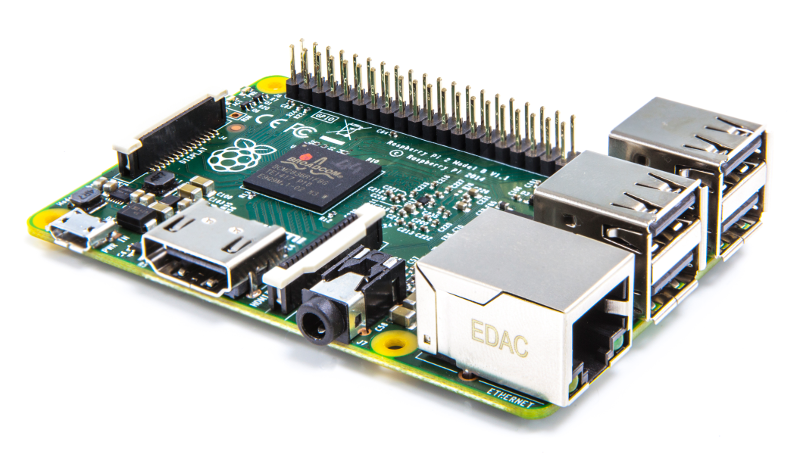
\includegraphics[width=5cm,natwidth=800,natheight=453]{rpi.png}
\end{figure}
\begin{itemize}
\item Petit ordinateur
\item Processeur ARM
\item 35 \$
\end{itemize}
\end{frame}

\section{Gestion du projet}

\begin{frame}
\frametitle{Gestion des ressources}
\begin{itemize}
\item 3 semaines
\item 3 personnes
\item 3 câbles USB-UART ( ~10 \euro{} pièce )
\item 3 Raspberry Pi 3 ( ~35 \euro{} pièce )
\item 2 Raspberry Pi 2 ( ~35 \euro{} pièce )
\end{itemize}
\end{frame}

\begin{frame}
\frametitle{Dépendances des tâches}
\begin{figure}[center]
\includegraphics[width=12cm,natwidth=915,natheight=511]{GrapheSpe.png}
\end{figure}
\end{frame}

\begin{frame}
\frametitle{Objectifs (1/3)}
\begin{figure}[center]
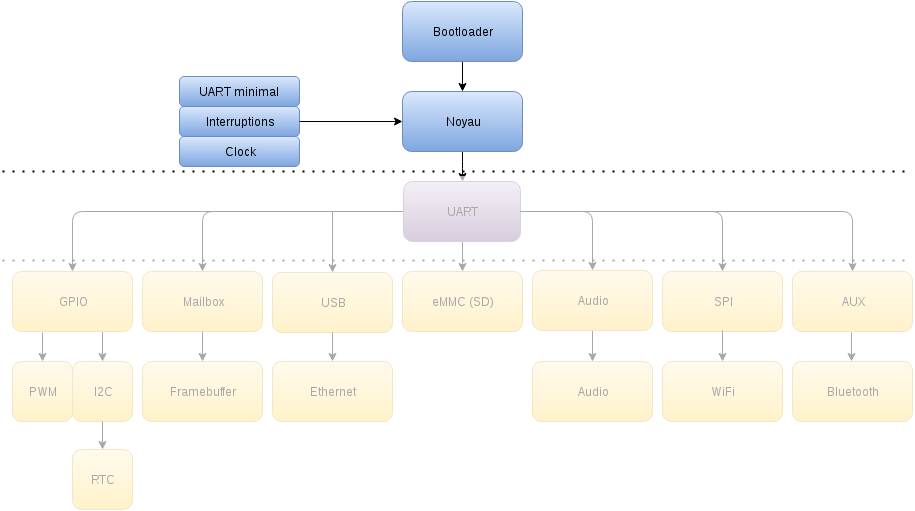
\includegraphics[width=7cm,natwidth=915,natheight=511]{GrapheSpe-1.png}
\end{figure}
Micro-noyau $\Rightarrow$ Système minimal
\begin{itemize}
\item UART minimal
\item Interruptions
\item Horloge
\end{itemize}
\end{frame}

\begin{frame}
\frametitle{Objectifs (2/3)}
\begin{figure}[center]
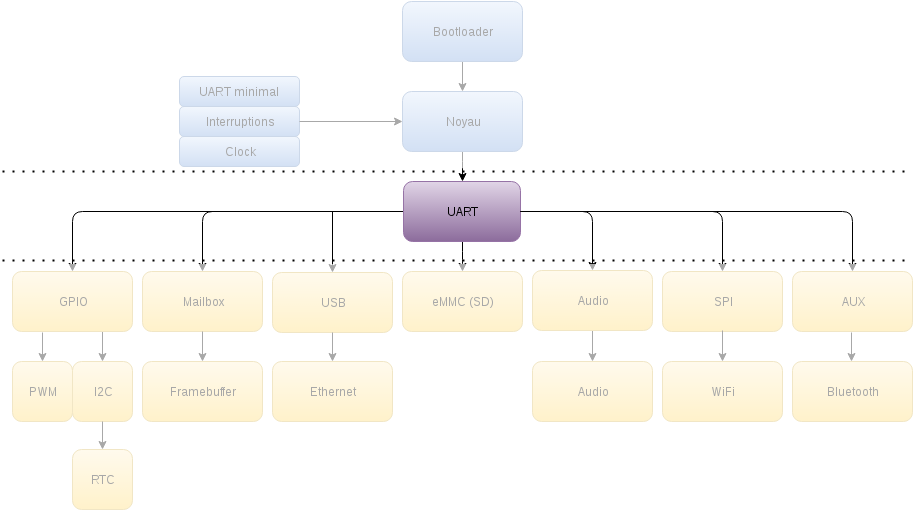
\includegraphics[width=7cm,natwidth=915,natheight=511]{GrapheSpe-2.png}
\end{figure}
UART $\Rightarrow$ Système interactif
\begin{figure}[center]
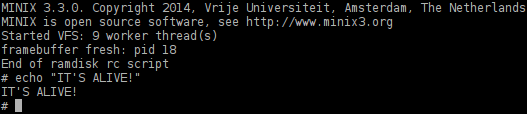
\includegraphics[width=12cm,natwidth=527,natheight=114]{console.png}
\end{figure}
\end{frame}

\begin{frame}
\frametitle{Objectifs (3/3)}
\begin{figure}[center]
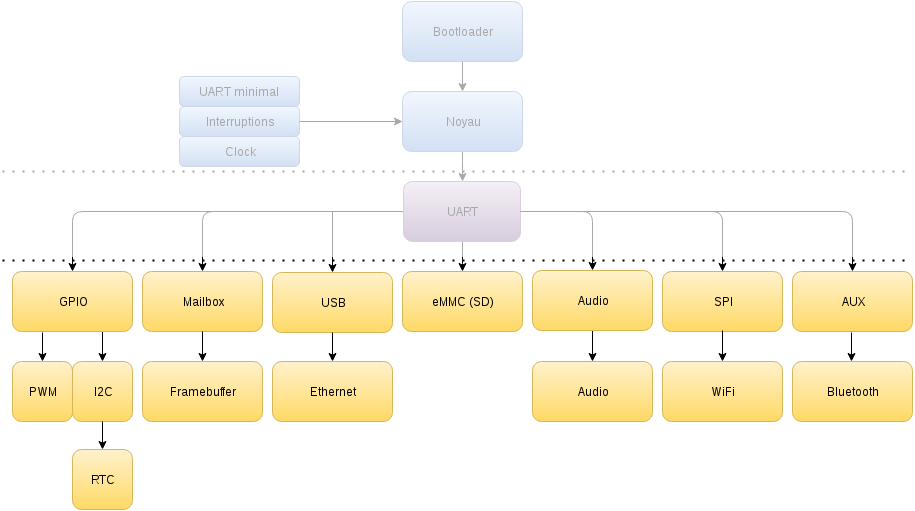
\includegraphics[width=7cm,natwidth=915,natheight=511]{GrapheSpe-3.png}
\end{figure}
Périphériques $\Rightarrow$ Système utile
\begin{itemize}
\item Framebuffer
\item GPIO
\item I2C
\item ...
\end{itemize}
\end{frame}

\section{Etat du projet}

\begin{frame}
\frametitle{Démonstration}
% \begin{figure}[center]
% 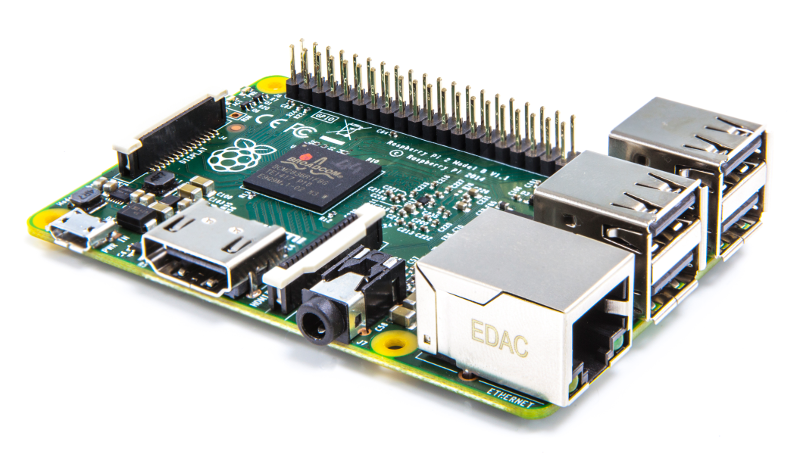
\includegraphics[width=5cm,natwidth=800,natheight=453]{rpi.png}
% \end{figure}
\begin{figure}[center]
\begin{Huge}
:-)
\end{Huge}
\end{figure}
\end{frame}

\begin{frame}
\frametitle{État d'avancement}

\begin{figure}[center]
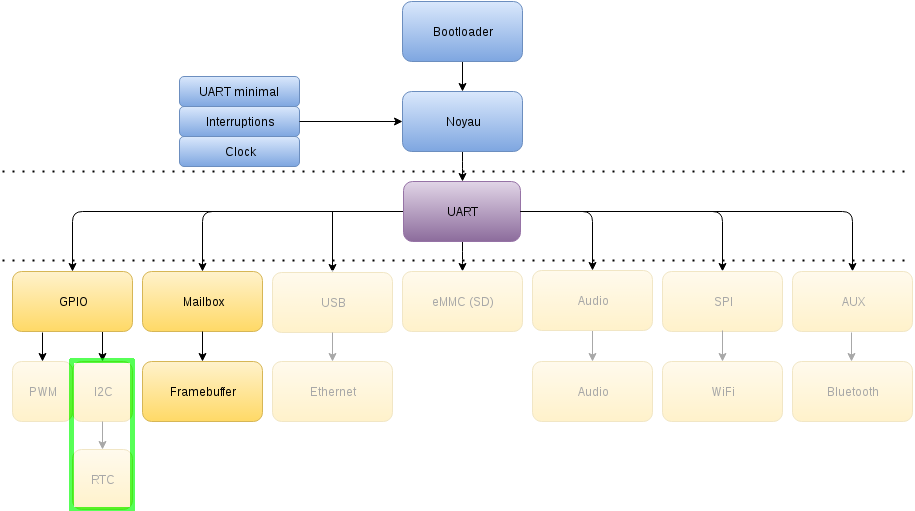
\includegraphics[width=7cm,natwidth=915,natheight=511]{GrapheSpe-4.png}
\end{figure}

\begin{columns}[T]

\begin{column}{.30\textwidth}
Fait :
\begin{itemize}
\item Micro-noyau
\item UART
\item Framebuffer
\item GPIO
\end{itemize}
\end{column}

\begin{column}{.30\textwidth}
À faire :
\begin{itemize}
\item I2C
\item RTC
\item ...
\end{itemize}
\end{column}

\end{columns}
\end{frame}

\begin{frame}
\frametitle{Conclusion}
\begin{itemize}
\item Difficultés
\item Flexibilité
\item Apprentisages
\end{itemize}
\end{frame}

\end{document}
